\documentclass{astroedu-lab}

\begin{document}

\pagestyle{plain}

\begin{problem}{\huge Лабораторная работа 2.4.1\\\\Определение теплоты испарения\\\\жидкости\\\\Выполнил Жданов Елисей Б01-205}

\section{Цель работы:}

1) Изучение петель гистерезиса различных ферромагнитных
материалов в переменных полях.


\section{Оборудование:}

Автотрансформатор, понижающий трансформатор,
интегрирующая цепочка, амперметр, вольтметр, электронный
осциллограф, делитель напряжения, тороидальные образцы с двумя обмотками.

\section{Теоретическая справка}

Ферромагнитные материалы часто применяются в трансформатоpax, дросселях, машинах переменного тока, то есть в устройствах, где они подвергаются периодическому перемагничиванию, - поэтому изучение магнитньх характеристик ферромагнетиков в переменньх полях представляет большой практический интерес. Основные характеристики ферромагнетиков - их коэрцитивное поле $H_c$, магнитная проницаемость $\mu$, рассеиваемая в виде тепла при перемагничивании мощность - зависят от частоты перемагничивающего поля. В данной работе кривые гистерезиса ферромагнитных материалов изучаются в поле частоты $\nu_0=50$ Гц с помощью электронного осциллографа.

\begin{figure}[!h]
	\centering
	\caption{Петля гистерезиса ферромагнетика}
	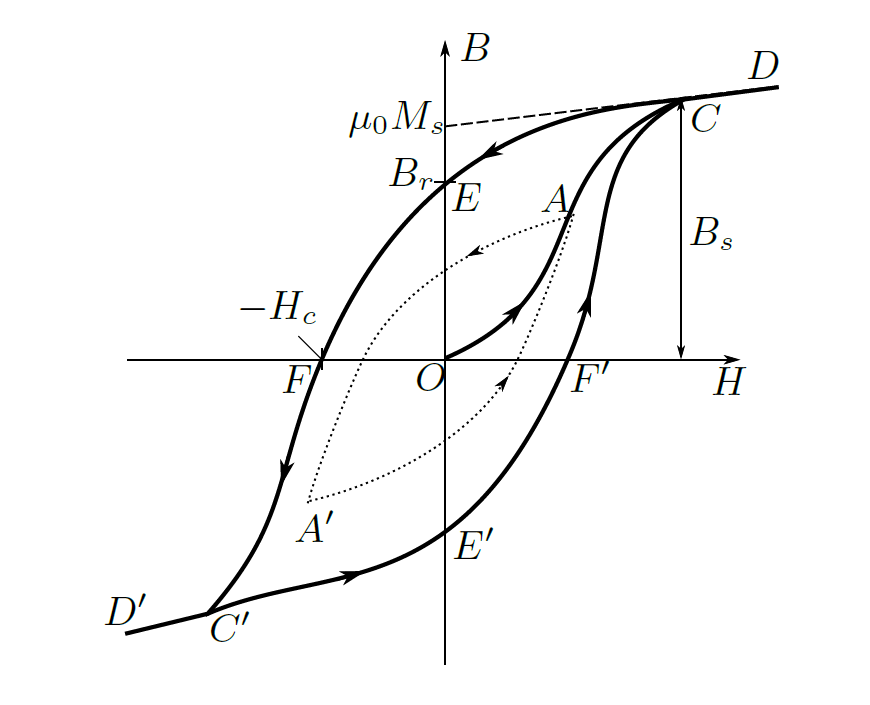
\includegraphics[width=0.5\textwidth]{theory.png}
	\label{fig:boiler}
\end{figure}

Магнитная индукция $B$ и напряжённость поля $H$ в ферромагнитном материале неоднозначно связаны между собой: индукция зависит не только от напряжённости, но и от предыстории образца. Связь между $B$ и $H$ типичного ферромагнетика иллюстрирует рис. 1 .

Если к ферромагнитному образцу прикладывать переменное внешнее магнитное поле, то его состояние на плоскости $H-B$ будет изменяться по замкнутой кривой - петле гистерезиса. Размер петли определяется максимальным значением напряжённости $H$ в цикле (напр., петля $\mathrm{AA}^{\prime}$, обозначенная пунктиром на рис. 1). Если амплитуда напряжённости достаточно велика, то образец будет периодически достигать насыщения, что на рисунке соответствует кривой $\mathrm{CEFC}^{\prime} \mathrm{E}^{\prime} \mathrm{F}^{\prime} \mathrm{C}$ (предельная петля гистерезиса). Пересечение предельной петли с вертикальной осью соответствует остаточной индукции $B_r$, пересечение с горизонтальной осью - коэрцитивному полю $H_c$. Крайние точки петель, соответствующие амплитудным значениям $H$ (например, точка А на рис. 1), лежат на начальной кривой намагничивания (OAC).

\subsection{Измерение магнитной индукции}

Магнитную индукцию $B$ удобно определять с помощью ЭДС, возникающей при изменении магнитного потока $\Phi$ в катушке, намотанной на образец. Пусть катушка с $N$ витками плотно охватывает образец сечением $S$, и индукция $B$ в образце однородна. Из формулы 4.20$)$ имеем
$$
|B|=\frac{1}{S N} \int \mathcal{E} d t
$$

Таким образом, для определения $B$ нужно проинтегрировать сигнал, наведённый меняющимся магнитным полем в измерительной катушке, намотанной на образец.

\begin{figure}[!h]
	\centering
	\caption{Интегрирующуая ячейка}
	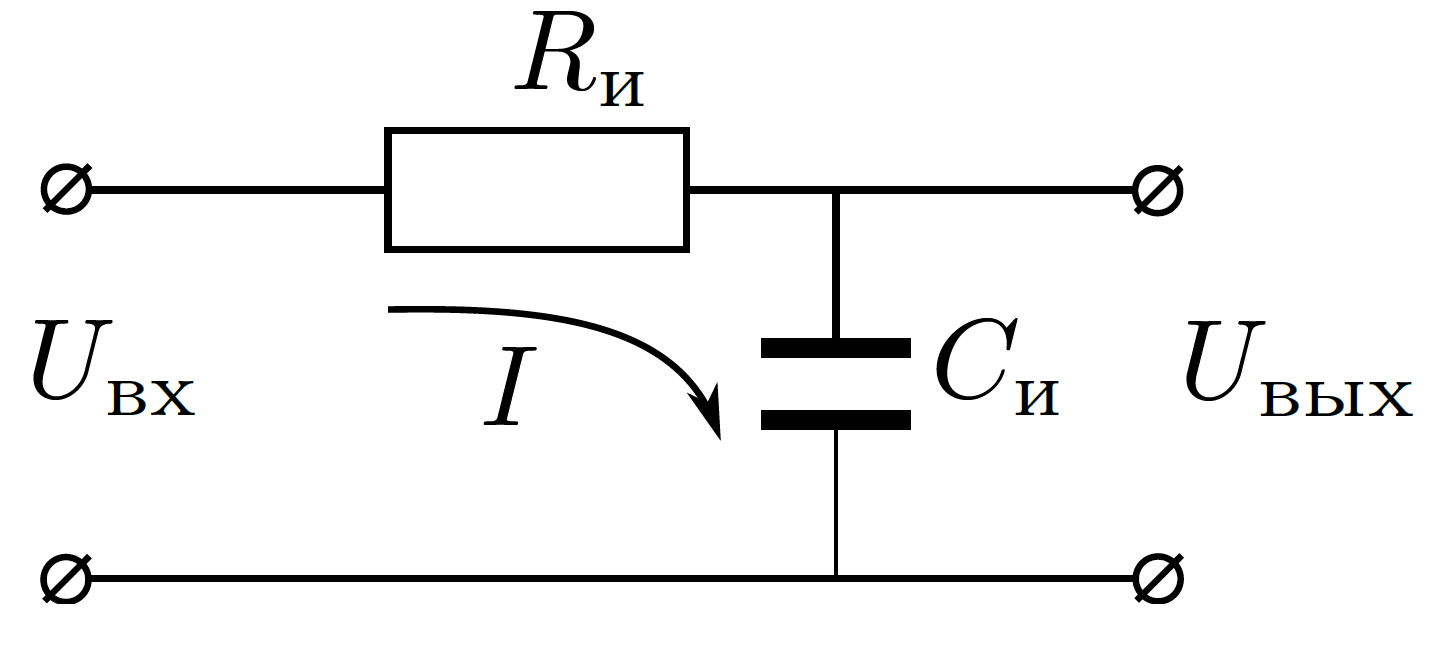
\includegraphics[width=0.5\textwidth]{theory2.png}
	\label{fig:boiler}
\end{figure}

Для интегрирования в работе используется интегрирующая $R C$-цепочка (рис. 2 ). «Входное» напряжение от источника $U_{\mathrm{Bx}}(t)$ подаётся на последовательно соединённые напряжение $U_{\text {вых }}(t)$ снимается с конденсатора. Предположим, что 1) сопротивление источника мало по сравнению с $\left.R_{\mathrm{n}}, 2\right)$ выходное сопротивление (сопротивление на входе осциллографа), напротив, велико: $R_{\text {вых }} \gg R_{\text {и }}$ и, наконец, 3) сопротивление $R_{\text {и }}$ достаточно велико, так что почти всё падение напряжения приходится на него, а $U_{\text {вых }} \ll U_{\mathrm{Bx}}$. В таком случае ток цепи равен $I=\left(U_{\mathrm{вx}}-U_{\mathrm{выx}}\right) / R_{\mathrm{n}} \approx U_{\mathrm{вx}} / R_{\mathrm{и}}$, и входное и выходное сопротивление связаны соотношением
$$
U_{\mathrm{Bux}}=\frac{q}{C_{\text {и }}}=\frac{1}{C_{\text {и }}} \int_0^t I d t \approx \frac{1}{\tau_{\text {и }}} \int_0^t U_{\mathrm{Bx}} d t .
$$

где $\tau_{\text {и }}=R_{\text {и }} C_{\text {и }}$ - постоянная времени $R C$-цепочки. Для индукции поля из (1) получаем
$$
|B|=\frac{1}{S N} \int U_{\mathrm{вx}} d t=\frac{\tau_{\text {и }}}{S N} U_{\text {вых }},
$$

\textbf{Замечание.} Уточним критерий применимости соотношения (2). Пусть на вход интегрирующей ячейки подан синусоидальный сигнал с частотой $\omega_0$. Тогда, пользуясь методом комплексньх амплитуд, нетрудно найти отношение амплитуд входного и вьходного напряжений:
$$
\frac{U_{\mathrm{Bsx}}}{U_{\mathrm{Bx}}}=\frac{1 /\left(\omega_0 C\right)}{\sqrt{R^2+\frac{1}{\left(\omega_0 C\right)^2}}}
$$

Видно, что неравенство $U_{\text {вых }} \ll U_{\text {вх }}$ реализуется, если
$$
\tau \equiv R C \gg \frac{1}{\omega_0}
$$
(импеданс конденсатора мал по сравнению сопротивлением резистора). В таком случае для синусоидального сигнала имеем
$$
\frac{U_{\mathrm{Bbx}}}{U_{\mathrm{Bx}}} \approx \frac{1}{\omega_0 \tau} .
$$

В общем случае, если $\omega_0$ - частота самой низкой гармоники в спектре произвольного входного сигнала, то при $\omega_0 \tau \gg 1$ неравенство $U_{\text {вых }} \ll U_{\mathrm{Bx}}$ выполняется на любой частоте $\omega>\omega_0$.

\section{Экспериментальная установка}

\begin{figure}[!h]
	\centering
	\caption{Схема установки для исследования намагричивания образцов}
	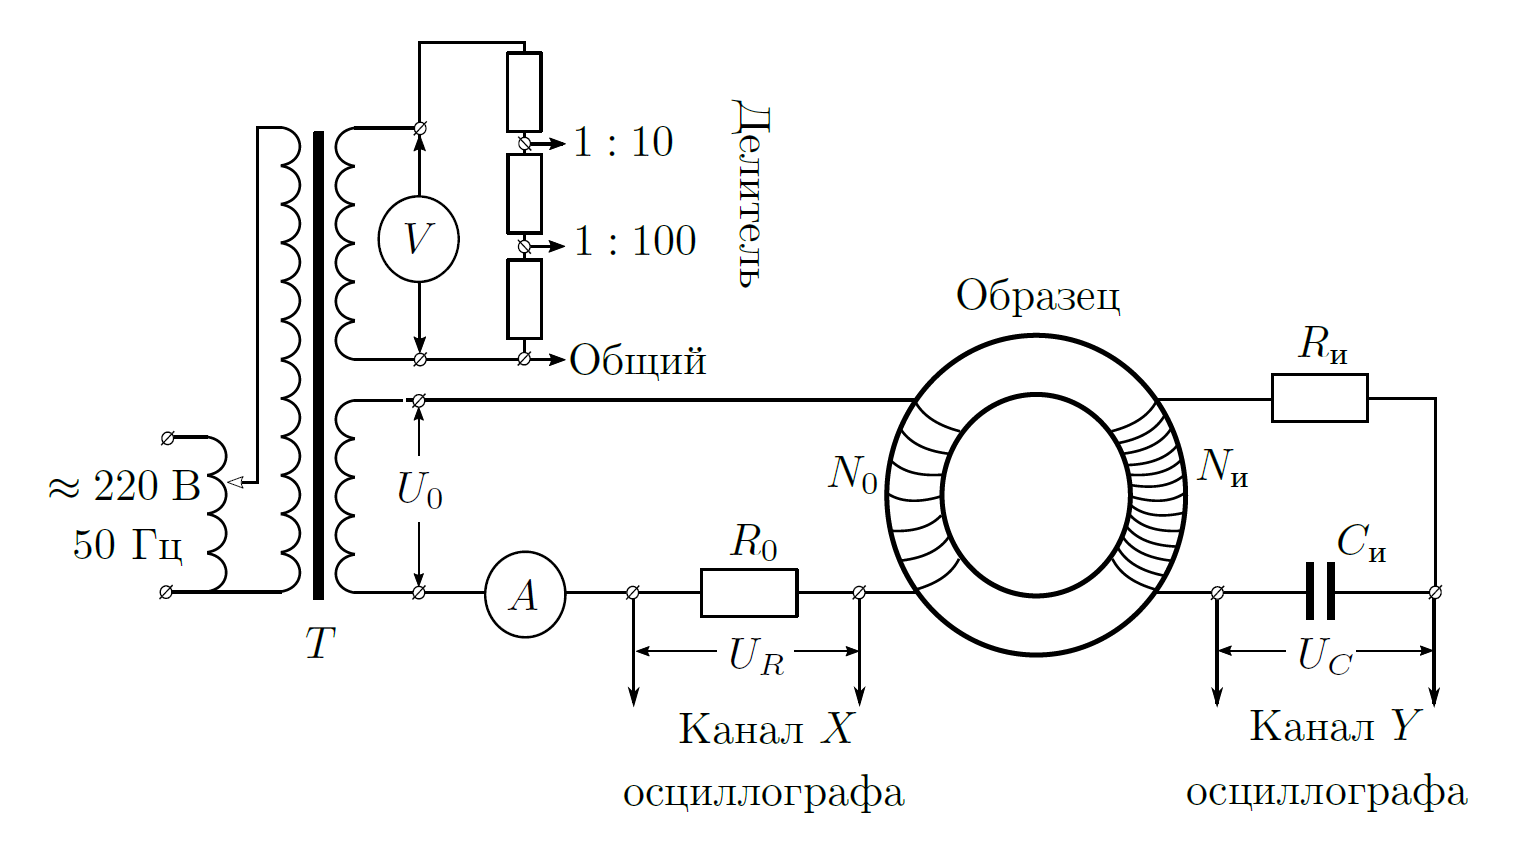
\includegraphics[width=0.9\textwidth]{установка.png}
	\label{fig:boiler}
\end{figure}

Схема установки изображена на рис. 3. Напряжение сети (220 В, 50 Гц) с помощью трансформаторного блока Т, состоящего из регулировочного автотрансформатора и разделительного понижающего трансформатора, подаётся на намагничивающую обмотку $N_0$ исследуемого образца.

В цепь намагничивающей катушки, на которую подаётся некоторое напряжение $U_0$, последовательно включено сопротивление $R_0$. Напряжение на $R_0$, равное $U_R=R_0 I_0$, где $I_0$ - ток в намагничивающей обмотке $N_0$, подаётся на канал $X$ осциллографа. Связь напряжённости $H$ в образце и тока $I_0$ рассчитывается по теореме о циркуляции (см. (4.16)).
238
Магнитные свойства вещества
Действующее значение переменного тока в обмотке $N_0$ измеряется амперметром $A$.

Для измерения магнитной индукции $B$ с измерительной обмотки $N_{\text {и }}$ на вход $R C$-цепочки подаётся напряжение $U_{\mathrm{n}}\left(U_{\mathrm{Bx}}\right)$, пропорциональное производной $d B / d t$. С интегрирующей ёмкости $C_{\text {и }}$ снимается напряжение $U_C\left(U_{\text {вых }}\right)$, пропорциональное величине $B$, и подаётся на вход $Y$ осциллографа. Значение индукции поля $B$ рассчитывается по формуле (3).

Замкнутая кривая, возникающая на экране, воспроизводит в некотором масштабе (различном для осей $X$ и $Y$ ) петлю гистерезиса. Чтобы придать этой кривой количественный смысл, необходимо установить масштабы изображения, т. е. провести калибровку каналов $X$ и $Y$ осциллографа.

\subsection{Калибровка осциллографа}

Калибровка канала $X$ осциллографа производится с помощью амперметра $A$. Предварительно необходимо закоротить обмотку $N_0$ (так как катушка с ферромагнитным образцом является нелинейным элементом, ток в ней не имеет синусоидальной формы, поэтому связать амплитуду тока с показаниями амперметра можно лишь с довольно большой погрешностью). При закороченной обмотке $N_0$ показания эффективного тока, умноженные на $2 \sqrt{2}$, дадут значение удвоенной амплитуды тока, подаваемого на ось $X$, соответствующего ширине горизонтальной развёртки на экране (осциллограф должен работать в режиме $X-Y)$.

Калибровка вертикальной оси $Y$, как правило, не нужна (переключатель масштабов осциллографа откалиброван при изготовлении - при условии, что ручка плавной регулировки находится в положении калибровки). Тем не менее, она может проводиться с помощью сигнала, снимаемого через делитель напряжения со второй катушки понижающего трансформатора (рис. 3). Вольтметр $V$ может достаточно точно измерить эффективное напряжение, подаваемое на вход осциллографа. После этого можно сравнить показания осциллографа и вольтметра.

\subsection{Измерение параметров интегрирующей ячейки}

Постоянную времени $R C$-цепочки можно определить экспериментально. С обмотки $U_0$ на вход интегрирующей цепочки подаётся синусоидальное напряжение с частотой цепи $\nu_0=\frac{\omega_0}{2 \pi}=50$ Гц. На вход $Y$ осциллографа или цифрового вольтметра поочерёдно подаются сигналы со входа $\left(U_{\mathrm{Bx}}=U_0\right)$ и выхода $\left(U_{\text {вых }}=U_C\right) R C$-цепочки. Измерив амплитуды этих сигналов, можно рассчитать постоянную времени $\tau_{\text {и }}=R_{\text {и }} C_{\text {и }}$ по формуле (5). Кроме того, сопротивление и ёмкость можно независимым образом измерить цифровым мультиметром.

\section{Измерения, Обработка}

\subsection{Измерение петли гистерезиса}

1) Соберем указанную схему

2) Проведем измерения для пермаллоя. Настроим критичесукю петлю гистерезиса.

3-5) Запишем коэффициенты в таблицу

6) Последовательно уменьшая амплитуду тока намагничивания, занесем значения всех крайних правых верхних точек А.

7) Приведу таблицу с параметрами пермаллоя и других сплавов.

\newpage

\begin{figure}[!h]
	\centering
	\caption{Петля гистерезиса для пермаллоя}
	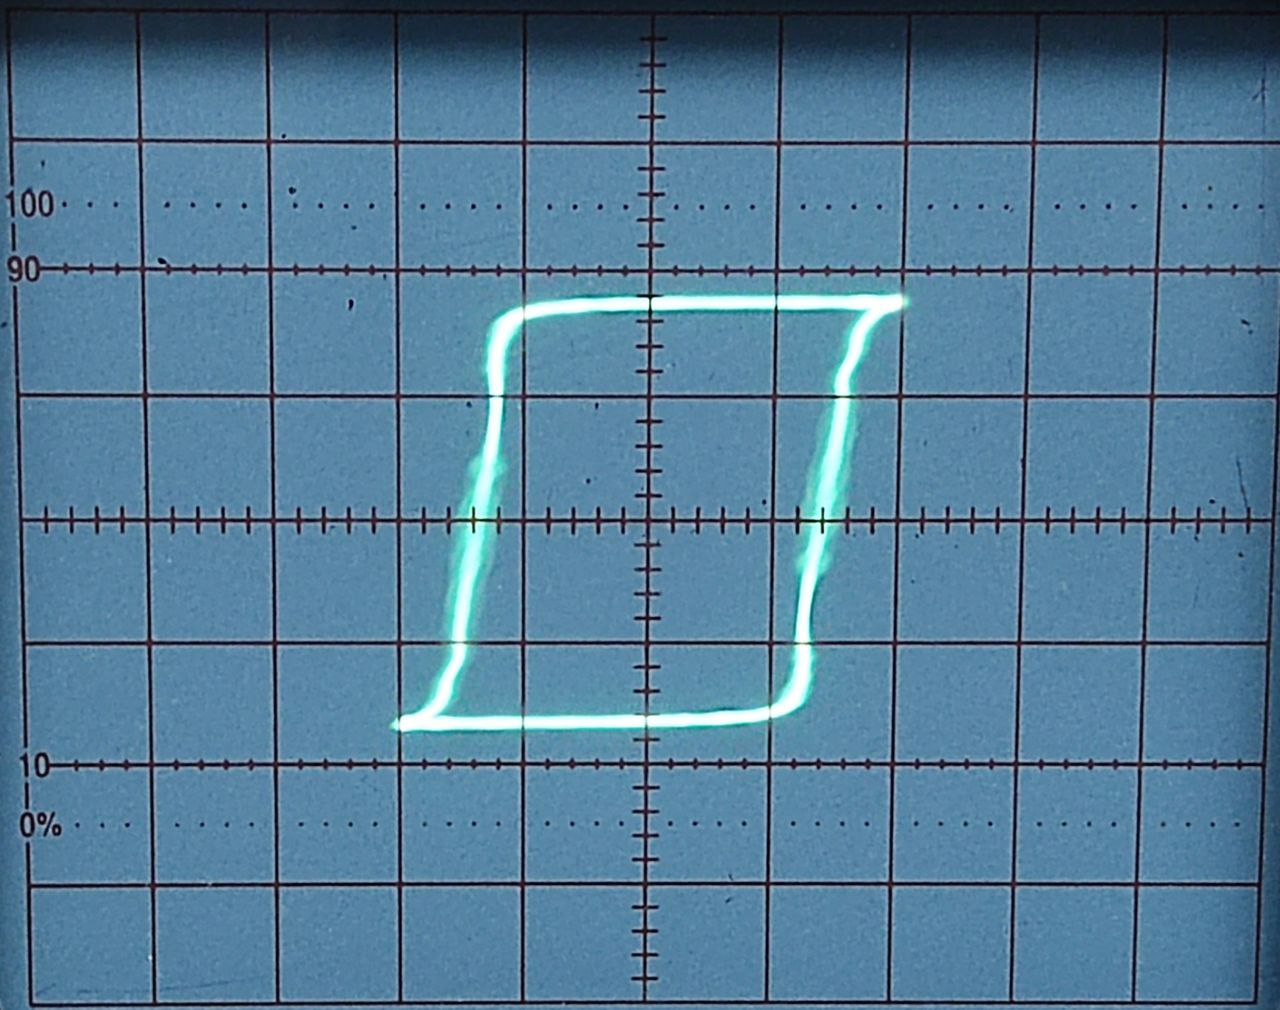
\includegraphics[width=0.8\textwidth]{loop1.jpg}
	\label{fig:boiler}
\end{figure}

.

\begin{figure}[!h]
	\centering
	\caption{Петля для кремнистого железа(похожая петля у феррита)}
	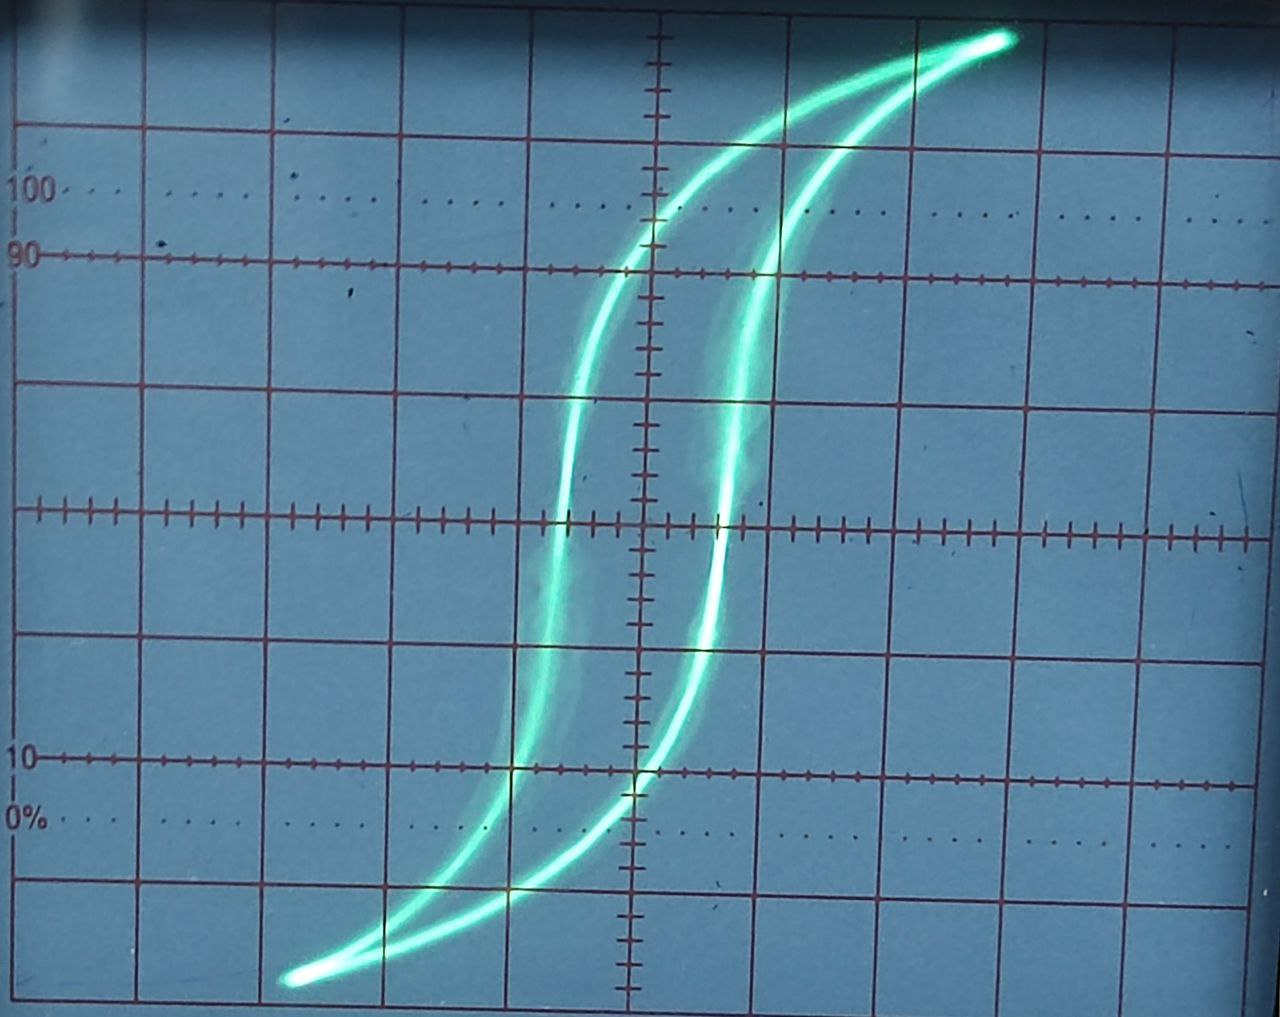
\includegraphics[width=0.8\textwidth]{loop2.jpg}
	\label{fig:boiler}
\end{figure}

\newpage

\begin{center}
\begin{tabular}{|c|c|c|c|}
\hline
& Пермаллой(Fe-Ni) & Кремнистое железо(Fe-Si) & Феррит(1000нн) \\
\hline
$2 X_s$, мВ & 160 & 720 & 108 \\
$2 Y_s$, мВ & 180 & 128 & 76  \\
$2 X_c$, мВ & 132 & 160 & 52  \\
$2 Y_c$, мВ & 170 & 56  & 13  \\
\hline
\end{tabular}
\end{center}

\begin{center}
\begin{tabular}{|c|c|c|c|}
\hline
& Пермаллой(Fe-Ni) & Кремнистое железо(Fe-Si) & Феррит(1000нн) \\
\hline
$N_0$, витков & 15   & 20  & 45  \\
$N_u$, витков & 300  & 200 & 400 \\
$S$, см$^2$   & 0.66 & 2   & 3	 \\
$2 \pi R$, см & 14.1 & 11  & 25  \\
\hline
\end{tabular}
\end{center}

\subsection{Калибровка осциллографа}

9-10) Проведем калибровку и занесем в таблицу реальные коэффициенты $K_x$ и $K_y$ для выбранных масштабов.

\begin{center}
\begin{tabular}{|c|c|c|c|}
\hline
канал & деления & $K_x$, мВ \\
\hline
5   мВ	& 6.1	& 2.74 \\
10  мВ	& 4.1	& 4.60 \\
20  мВ 	& 4.3	& 9.67 \\
50  мВ	& 4.0	& 24.7 \\
100 мВ	& 4.4	& 56.0 \\ 
\hline
\end{tabular}
\end{center}

\begin{center}
\begin{tabular}{|c|c|c|c|}
\hline
канал & деления & U, мВ & $K_y$, мВ \\
\hline
5  мВ	& 3	& 9.7	& 4.57 \\
10 мВ	& 3	& 20.3	& 9.5  \\
20 мВ 	& 3	& 40.1	& 19   \\
50 мВ	& 3	& 101.4	& 47   \\
\hline
\end{tabular}
\end{center}

Как видим, канал Y не нуждается в пересчете, поскольку откалиброван собственно, в погрешности измеряемых калибровочных величин. По каналу же X пересчет должен производиться.

\subsection{Определение параметров RC-ячейки}

11-12) $U_\text{вх} = 3.3$ В. $U_\text{вых} = 0.027$ В. $\nu_0 = 50$ Гц. Тогда $\tau = \frac{U_\text{вых}}{\omega_0 U_\text{вх}} = \frac{U_\text{вых}}{2 \pi \nu_0 \cdot U_\text{вх}} \approx 0.39$ сек

13) $\tau = R C = 0.4$ сек, что приблизительно совпадает с расчетом через напряжения.

\subsection{Обработка результатов}

14) Из теории:

\begin{equation}
	H = \frac{I N_0}{2 \pi R} = \frac{U_X N_0}{2 \pi R R_0}
\end{equation}

\begin{equation}
	B = \mu \mu_0 H = \frac{R_u C_u U_Y}{S N_u}
\end{equation}

В реальности необходимо учесть калибровку, домножив подставляемое напряжение на $\frac{K_x}{R_x}$, $R_x$ - шаг режима ЭО. Для OY этот коэффициент - единица, а для OX: $\approx 0.5$.

15-16) Занесем полученные коэффициенты в таблицу

\begin{center}
\begin{tabular}{|c|c|c|c|}
\hline
& Пермаллой(Fe-Ni) & Кремнистое железо(Fe-Si) & Феррит(1000нн) \\
\hline
$H_{max}$, $\frac{\text{А}}{\text{м}}$ & 42.6 &	327 &	48.6  \\
$B_s$, Тс & 3.64	& 1.28 &	0.253 \\
$H_c$, $\frac{\text{А}}{\text{м}}$ & 35.1&	72.7&	23.4	 \\
$B_r$, Тс & 3.44 &	0.56 &	0.043  \\
\hline
\end{tabular}
\end{center}

17) Построим кривые для всех 3-х материалов на графике

\begin{figure}[!h]
	\centering
	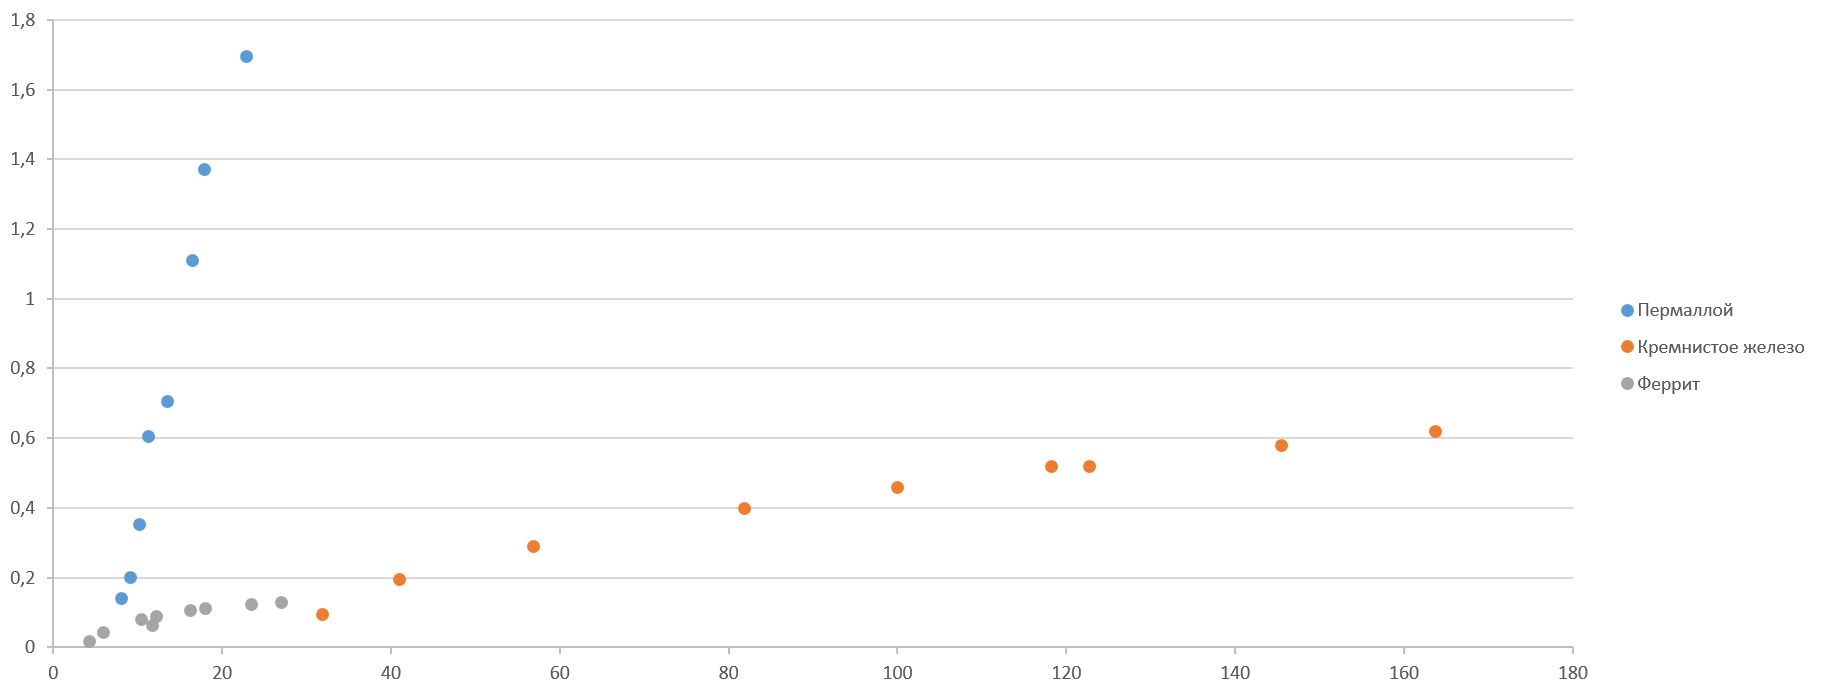
\includegraphics[width=1\textwidth]{график.png}
	\label{fig:boiler}
\end{figure}

Найдем угловые коэффициенты прямых для установки по МНК.

\[
	a = \frac{<x_i y_i> - < x > < y_i >}{< x_i^2> - < x_i >^2}
\]

\[
	b = < \nu_i > - a < N_i >
\]

Также рассчитаем их погрешности

\begin{equation}
	S_a^2 = \frac{< x_i^2>}{< x_i^2 > - < x_i >^2} \cdot \frac{<  b_i - b > ^2}{n - 2}
\end{equation}

По измеренным данным трудно рассчитать начальное и максимальное значение дифференциальной магнитной проницаемости, поэтому приведу среднее характерное значение

Для феррита $\mu_\text{дифф} = 0.110 \pm  0.007$, для кремниевого железа $\mu_\text{дифф} = 0.0038 \pm 0.0003$, для феррита $\mu_\text{дифф} = 0.0046 \pm 0.0007$

\section{Вывод}

Полученные значения в целом порой, очень даже неплохо совпадают с табличными значениями для материалов. Понятное дело, для точного расчета той-же дифференциальной магнитной проницаемости требуется большое количество точек и, возможно, дифференцирующая цепочка. Но при соответствующем качестве эксперимента полученные значения выходят довольно вразумительными.

\section{Ресурсы}

Расчет по МНК: метод-наименьших-квадратов.рф


\end{problem}
\end{document}